\paragraph{Stimuli.} We used 64 equally spaced stimuli that varied only in hue in CIELUV space. 

\paragraph{4-Alternative Forced Choice (4-AFC): Non-human primates.} Non-human primates were trained on a color-matching task. Trials begin with fixation (50 ms) on a white cross in the center of the screen. A cue stimulus (colored disc) is shown to one side of the fixation cross (750 ms). The position of the cue is invariant throughout a daily session. Following cue presentation, the monkey must maintain fixation (600-900 ms) before the choice stimuli appear on the screen alongside the fixation cross (500-1000 ms). The choices are positioned at constant eccentricity and with equal spacing in the hemifield opposite the cue stimulus, with the exact positions of the stimuli varying randomly trial-to-trial. One choice is always a direct match to the cue, and the other three are randomly sampled. Upon offset of the fixation cross, the animal makes a selection by saccade, and is rewarded for selecting the choice that is identical to the cue. 

\paragraph{4-Alternative Forced Choice: Human participants.} Human participants were recruited via Amazon Mechanical Turk to perform an analogous version of the non-human primate 4-AFC task. Participants click on an initial fixation cross to request a trial, after which a cue is shown to one side of the fixation cross (750 ms). After cue offset, a fixation cross is shown and the cursor is hidden to de-incentivize mouse movement (1500 ms). Four choices are then shown, and participants make their selection by clicking. 

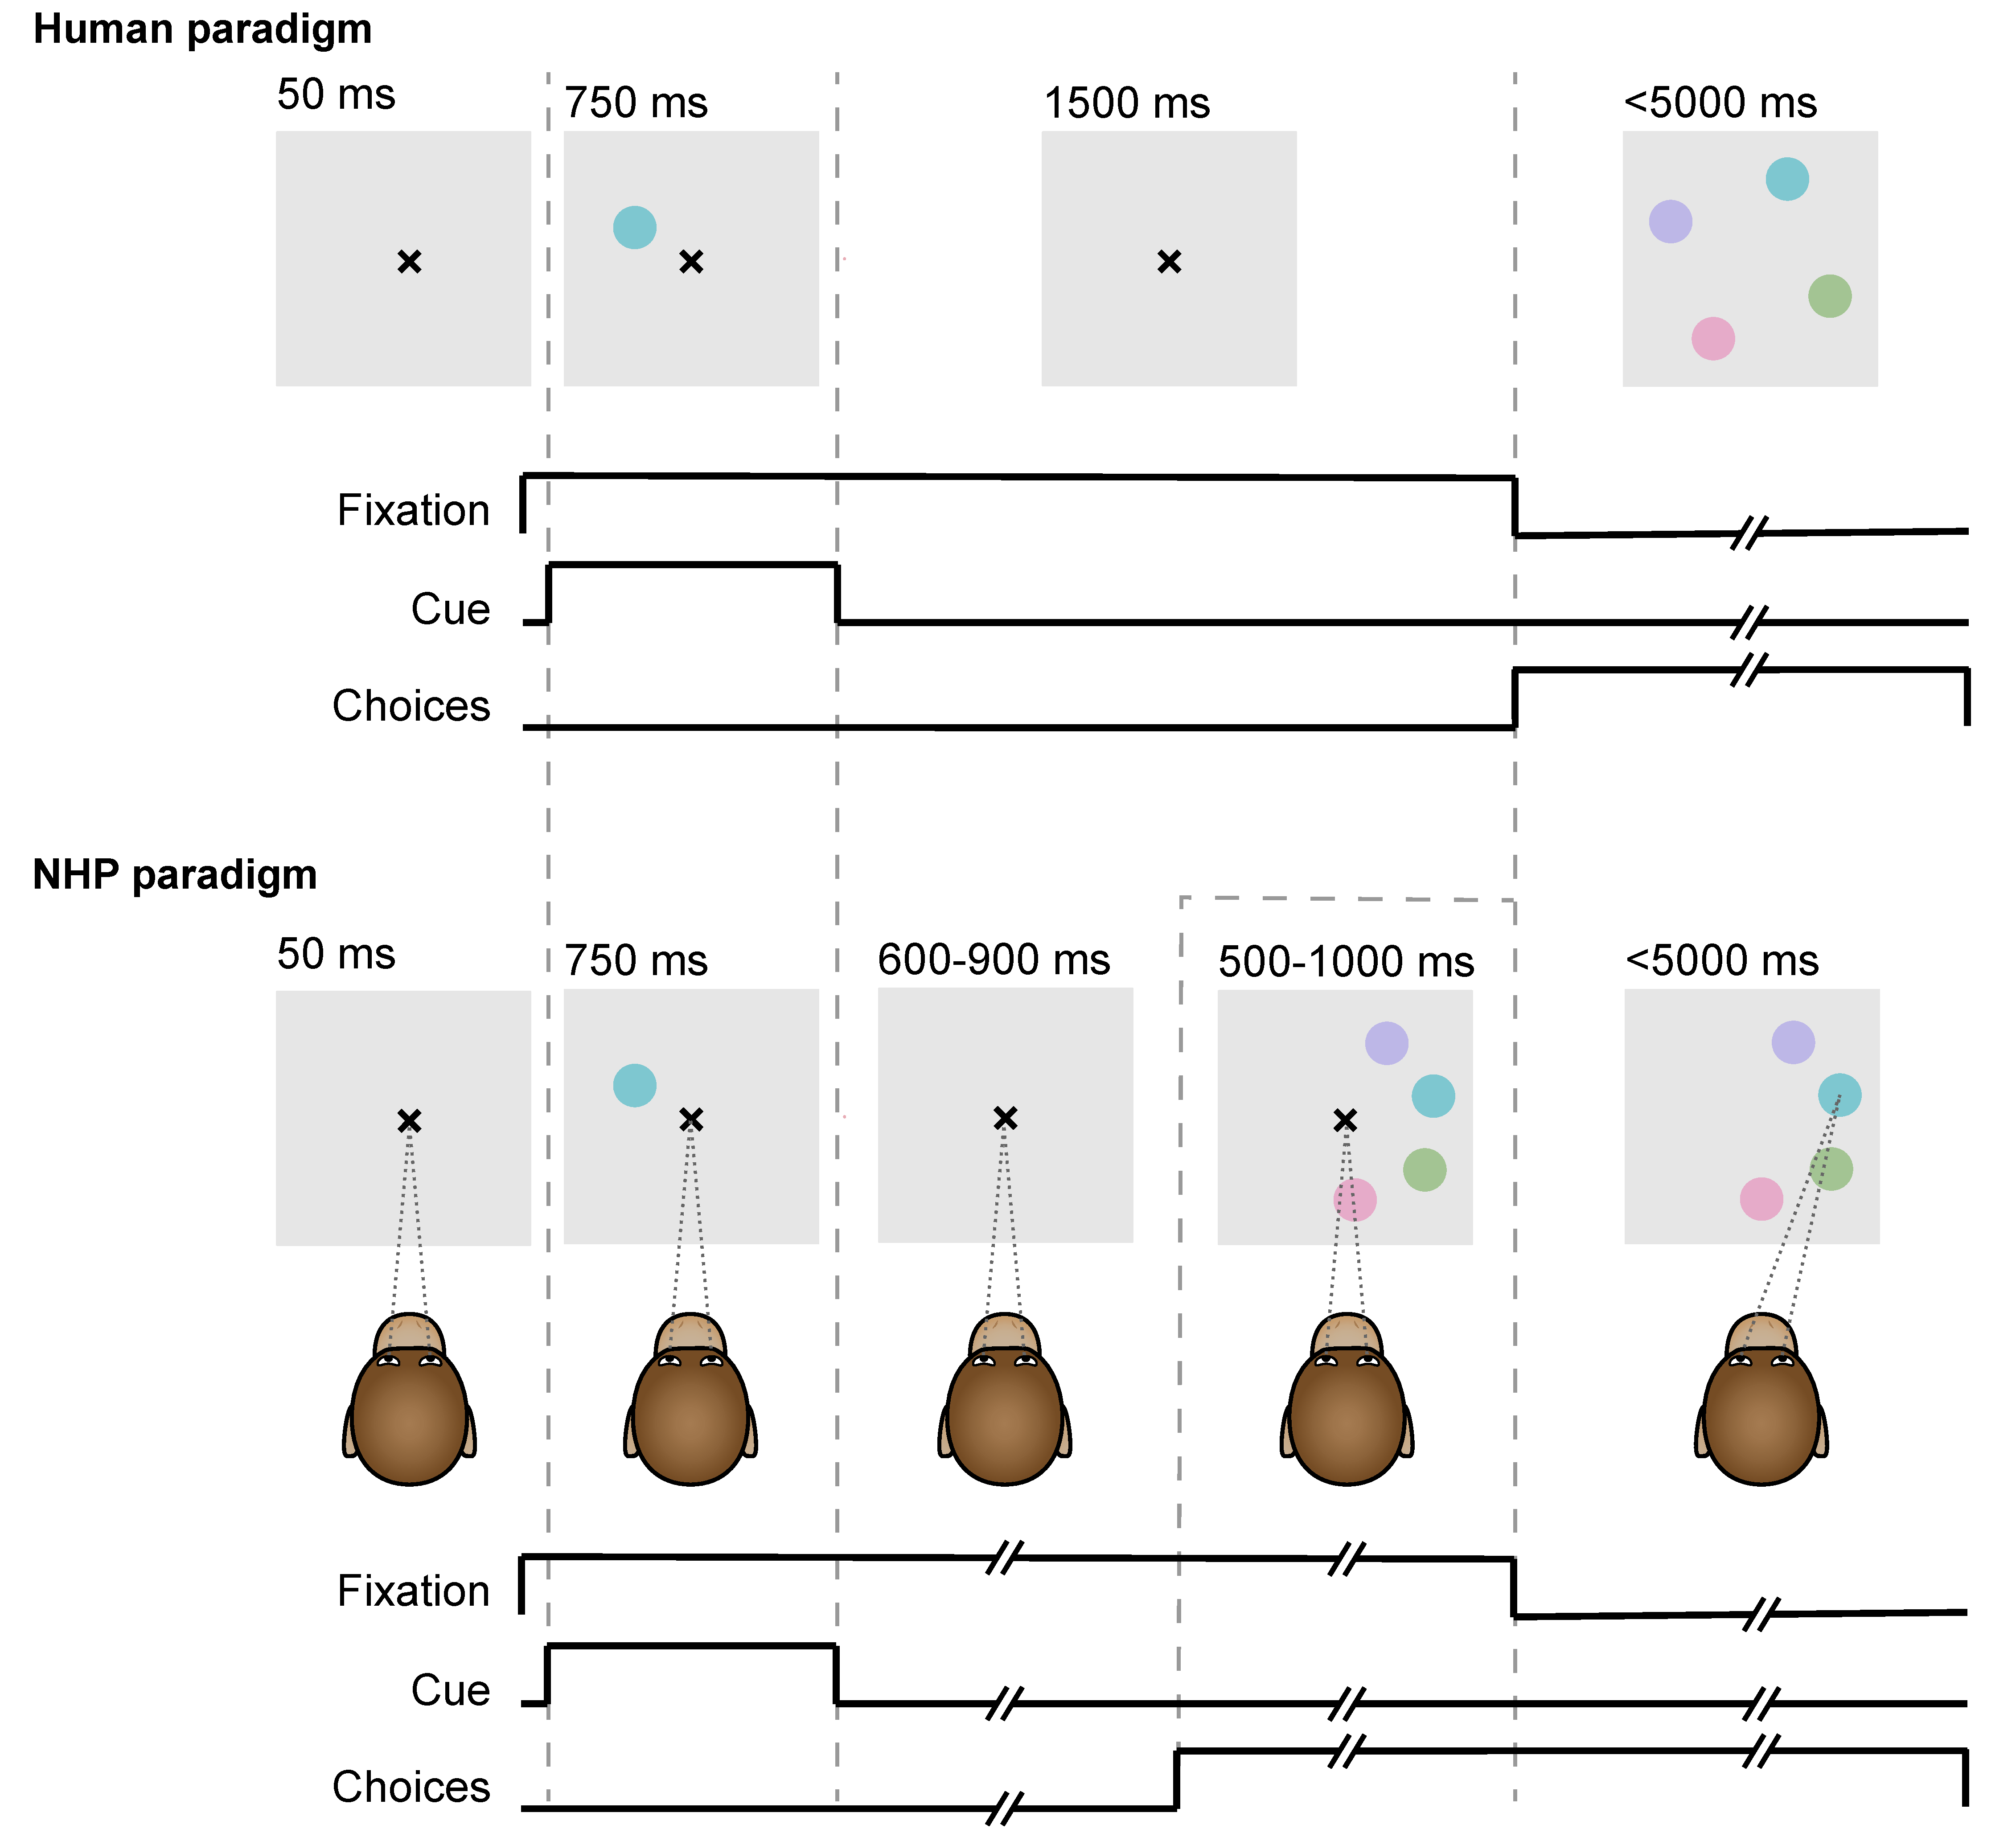
\includegraphics[width=300]{paradigm.pdf}

\paragraph{_Figure X._} 4-Alternative Forced Choice (4-AFC) Paradigm. 

\paragraph{Color-naming task} 


